%%
%% Automatically generated file from DocOnce source
%% (https://github.com/hplgit/doconce/)
%%

% #define PREAMBLE

% #ifdef PREAMBLE
%-------------------- begin preamble ----------------------

\documentclass[%
oneside,                 % oneside: electronic viewing, twoside: printing
final,                   % draft: marks overfull hboxes, figures with paths
10pt]{article}

\listfiles               %  print all files needed to compile this document

\usepackage{relsize,makeidx,color,setspace,amsmath,amsfonts,amssymb}
\usepackage[table]{xcolor}
\usepackage{bm,ltablex,microtype}

\usepackage[pdftex]{graphicx}

% Packages for typesetting blocks of computer code
\usepackage{fancyvrb,framed,moreverb}

% Define colors
\definecolor{orange}{cmyk}{0,0.4,0.8,0.2}
\definecolor{tucorange}{rgb}{1.0,0.64,0}
\definecolor{darkorange}{rgb}{.71,0.21,0.01}
\definecolor{darkgreen}{rgb}{.12,.54,.11}
\definecolor{myteal}{rgb}{.26, .44, .56}
\definecolor{gray}{gray}{0.45}
\definecolor{mediumgray}{gray}{.8}
\definecolor{lightgray}{gray}{.95}
\definecolor{brown}{rgb}{0.54,0.27,0.07}
\definecolor{purple}{rgb}{0.5,0.0,0.5}
\definecolor{darkgray}{gray}{0.25}
\definecolor{darkblue}{rgb}{0,0.08,0.45}
\definecolor{darkblue2}{rgb}{0,0,0.8}
\definecolor{lightred}{rgb}{1.0,0.39,0.28}
\definecolor{lightgreen}{rgb}{0.48,0.99,0.0}
\definecolor{lightblue}{rgb}{0.53,0.81,0.92}
\definecolor{lightblue2}{rgb}{0.3,0.3,1.0}
\definecolor{lightpurple}{rgb}{0.87,0.63,0.87}
\definecolor{lightcyan}{rgb}{0.5,1.0,0.83}

\colorlet{comment_green}{green!50!black}
\colorlet{string_red}{red!60!black}
\colorlet{keyword_pink}{magenta!70!black}
\colorlet{indendifier_green}{green!70!white}

% Backgrounds for code
\definecolor{cbg_gray}{rgb}{.95, .95, .95}
\definecolor{bar_gray}{rgb}{.92, .92, .92}

\definecolor{cbg_yellowgray}{rgb}{.95, .95, .85}
\definecolor{bar_yellowgray}{rgb}{.95, .95, .65}

\colorlet{cbg_yellow2}{yellow!10}
\colorlet{bar_yellow2}{yellow!20}

\definecolor{cbg_yellow1}{rgb}{.98, .98, 0.8}
\definecolor{bar_yellow1}{rgb}{.98, .98, 0.4}

\definecolor{cbg_red1}{rgb}{1, 0.85, 0.85}
\definecolor{bar_red1}{rgb}{1, 0.75, 0.85}

\definecolor{cbg_blue1}{rgb}{0.87843, 0.95686, 1.0}
\definecolor{bar_blue1}{rgb}{0.7,     0.95686, 1}

%\setlength{\fboxsep}{-1.5mm}  % adjust cod_vpad/pro_vpad background box

%% Background for code blocks (parameter is color name)

%% pro/cod_vpad: gives some vertical padding before and after the text
%% (but has more simplistic code than _cod/pro_tight+cod/pro).
%% pro/cod_vpad can be used to enclose Verbatim or lst begin/end for code.
%% pro/cod calls _pro/cod_tight and has very little vertical padding,
%% used to enclose Verbatim and other begin/end for code.
%% (pro/cod is what the ptex2tex program could produce with the
%% Blue/BlueBar definitions in .ptex2tex.cfg.)

\newenvironment{cod_vpad}[1]{
   \def\FrameCommand{\colorbox{#1}}
   \MakeFramed{\FrameRestore}}
   {\endMakeFramed}

\newenvironment{_cod_tight}[1]{
   \def\FrameCommand{\colorbox{#1}}
   \FrameRule0.6pt\MakeFramed {\FrameRestore}\vskip3mm}
   {\vskip0mm\endMakeFramed}

\newenvironment{cod}[1]{
\bgroup\rmfamily
\fboxsep=0mm\relax
\begin{_cod_tight}{#1}
\list{}{\parsep=-2mm\parskip=0mm\topsep=0pt\leftmargin=2mm
\rightmargin=2\leftmargin\leftmargin=4pt\relax}
\item\relax}
{\endlist\end{_cod_tight}\egroup}

%% Background for complete program blocks (parameter 1 is color name
%% for background, parameter 2 is color for left bar)
\newenvironment{pro_vpad}[2]{
   \def\FrameCommand{\color{#2}\vrule width 1mm\normalcolor\colorbox{#1}}
   \MakeFramed{\FrameRestore}}
   {\endMakeFramed}

\newenvironment{_pro_tight}[2]{
   \def\FrameCommand{\color{#2}\vrule width 1mm\normalcolor\colorbox{#1}}
   \FrameRule0.6pt\MakeFramed {\advance\hsize-2mm\FrameRestore}\vskip3mm}
   {\vskip0mm\endMakeFramed}

\newenvironment{pro}[2]{
\bgroup\rmfamily
\fboxsep=0mm\relax
\begin{_pro_tight}{#1}{#2}
\list{}{\parsep=-2mm\parskip=0mm\topsep=0pt\leftmargin=2mm
\rightmargin=2\leftmargin\leftmargin=4pt\relax}
\item\relax}
{\endlist\end{_pro_tight}\egroup}

\usepackage{minted}
\usemintedstyle{default}

\usepackage[T1]{fontenc}
%\usepackage[latin1]{inputenc}
\usepackage{ucs}
\usepackage[utf8x]{inputenc}

\usepackage{lmodern}         % Latin Modern fonts derived from Computer Modern

% Hyperlinks in PDF:
\definecolor{linkcolor}{rgb}{0,0,0.4}
\usepackage{hyperref}
\hypersetup{
    breaklinks=true,
    colorlinks=true,
    linkcolor=linkcolor,
    urlcolor=linkcolor,
    citecolor=black,
    filecolor=black,
    %filecolor=blue,
    pdfmenubar=true,
    pdftoolbar=true,
    bookmarksdepth=3   % Uncomment (and tweak) for PDF bookmarks with more levels than the TOC
    }
%\hyperbaseurl{}   % hyperlinks are relative to this root

\setcounter{tocdepth}{2}  % levels in table of contents

% Tricks for having figures close to where they are defined:
% 1. define less restrictive rules for where to put figures
\setcounter{topnumber}{2}
\setcounter{bottomnumber}{2}
\setcounter{totalnumber}{4}
\renewcommand{\topfraction}{0.95}
\renewcommand{\bottomfraction}{0.95}
\renewcommand{\textfraction}{0}
\renewcommand{\floatpagefraction}{0.75}
% floatpagefraction must always be less than topfraction!
% 2. ensure all figures are flushed before next section
\usepackage[section]{placeins}
% 3. enable begin{figure}[H] (often leads to ugly pagebreaks)
%\usepackage{float}\restylefloat{figure}

% --- fancyhdr package for fancy headers ---
\usepackage{fancyhdr}
\fancyhf{} % sets both header and footer to nothing
\renewcommand{\headrulewidth}{0pt}
\fancyfoot[LE,RO]{\thepage}
% Ensure copyright on titlepage (article style) and chapter pages (book style)
\fancypagestyle{plain}{
  \fancyhf{}
  \fancyfoot[C]{{\footnotesize \copyright\ 2021, Ahmed Ammar. Released under CC Attribution 4.0 license}}
%  \renewcommand{\footrulewidth}{0mm}
  \renewcommand{\headrulewidth}{0mm}
}
% Ensure copyright on titlepages with \thispagestyle{empty}
\fancypagestyle{empty}{
  \fancyhf{}
  \fancyfoot[C]{{\footnotesize \copyright\ 2021, Ahmed Ammar. Released under CC Attribution 4.0 license}}
  \renewcommand{\footrulewidth}{0mm}
  \renewcommand{\headrulewidth}{0mm}
}

\pagestyle{fancy}


\usepackage{framed,wrapfig}

% --- begin definitions of admonition environments ---

% Admonition style "grayicon" has colored background, no frame, and an icon
% Admon "notice"
\definecolor{grayicon_notice_background}{rgb}{0.91,0.91,0.91}
% \fboxsep sets the space between the text and the box
\newenvironment{noticeshaded}
{\def\FrameCommand{\fboxsep=3mm\colorbox{grayicon_notice_background}}
 \MakeFramed {\advance\hsize-\width \FrameRestore}}{\endMakeFramed}

\newenvironment{notice_grayiconadmon}[1][Note]{
\begin{noticeshaded}
\noindent
\begin{wrapfigure}{l}{0.07\textwidth}
\vspace{-13pt}

\includegraphics[width=0.07\textwidth]{latex_figs/small_gray_notice}
\end{wrapfigure} \textbf{#1}\par
\nobreak\noindent\ignorespaces
}
{
\end{noticeshaded}
}

% Admonition style "grayicon" has colored background, no frame, and an icon
% Admon "summary"
\definecolor{grayicon_summary_background}{rgb}{0.91,0.91,0.91}
% \fboxsep sets the space between the text and the box
\newenvironment{summaryshaded}
{\def\FrameCommand{\fboxsep=3mm\colorbox{grayicon_summary_background}}
 \MakeFramed {\advance\hsize-\width \FrameRestore}}{\endMakeFramed}

\newenvironment{summary_grayiconadmon}[1][Résumé]{
\begin{summaryshaded}
\noindent
\begin{wrapfigure}{l}{0.07\textwidth}
\vspace{-13pt}
\includegraphics[width=0.07\textwidth]{latex_figs/small_gray_summary}
\end{wrapfigure} \textbf{#1}\par
\nobreak\noindent\ignorespaces
}
{
\end{summaryshaded}
}

% Admonition style "grayicon" has colored background, no frame, and an icon
% Admon "warning"
\definecolor{grayicon_warning_background}{rgb}{0.91,0.91,0.91}
% \fboxsep sets the space between the text and the box
\newenvironment{warningshaded}
{\def\FrameCommand{\fboxsep=3mm\colorbox{grayicon_warning_background}}
 \MakeFramed {\advance\hsize-\width \FrameRestore}}{\endMakeFramed}

\newenvironment{warning_grayiconadmon}[1][Avertissement]{
\begin{warningshaded}
\noindent
\begin{wrapfigure}{l}{0.07\textwidth}
\vspace{-13pt}
\includegraphics[width=0.07\textwidth]{latex_figs/small_gray_warning}
\end{wrapfigure} \textbf{#1}\par
\nobreak\noindent\ignorespaces
}
{
\end{warningshaded}
}

% Admonition style "grayicon" has colored background, no frame, and an icon
% Admon "question"
\definecolor{grayicon_question_background}{rgb}{0.91,0.91,0.91}
% \fboxsep sets the space between the text and the box
\newenvironment{questionshaded}
{\def\FrameCommand{\fboxsep=3mm\colorbox{grayicon_question_background}}
 \MakeFramed {\advance\hsize-\width \FrameRestore}}{\endMakeFramed}

\newenvironment{question_grayiconadmon}[1][Question]{
\begin{questionshaded}
\noindent
\begin{wrapfigure}{l}{0.07\textwidth}
\vspace{-13pt}

\includegraphics[width=0.07\textwidth]{latex_figs/small_gray_question2}
\end{wrapfigure} \textbf{#1}\par
\nobreak\noindent\ignorespaces
}
{
\end{questionshaded}
}

% Admonition style "grayicon" has colored background, no frame, and an icon
% Admon "block"
\definecolor{grayicon_block_background}{rgb}{0.91,0.91,0.91}
% \fboxsep sets the space between the text and the box
\newenvironment{blockshaded}
{\def\FrameCommand{\fboxsep=3mm\colorbox{grayicon_block_background}}
 \MakeFramed {\advance\hsize-\width \FrameRestore}}{\endMakeFramed}

\newenvironment{block_grayiconadmon}[1][Block]{
\begin{blockshaded}
\noindent
 \textbf{#1}\par
\nobreak\noindent\ignorespaces
}
{
\end{blockshaded}
}

% --- end of definitions of admonition environments ---

% prevent orhpans and widows
\clubpenalty = 10000
\widowpenalty = 10000

% --- end of standard preamble for documents ---


% insert custom LaTeX commands...

\raggedbottom
\makeindex
\usepackage[totoc]{idxlayout}   % for index in the toc
\usepackage[nottoc]{tocbibind}  % for references/bibliography in the toc

%-------------------- end preamble ----------------------

\begin{document}

% matching end for #ifdef PREAMBLE
% #endif

\newcommand{\exercisesection}[1]{\subsection*{#1}}


% ------------------- main content ----------------------



% ----------------- title -------------------------

\thispagestyle{empty}

\begin{center}
{\LARGE\bf
\begin{spacing}{1.25}
Intégration numérique
\end{spacing}
}
\end{center}

% ----------------- author(s) -------------------------

\begin{center}
{\bf Ahmed Ammar (\texttt{ahmed.ammar@fst.utm.tn})}
\end{center}

    \begin{center}
% List of all institutions:
\centerline{{\small Institut Préparatoire aux Études Scientifiques et Techniques, Université de Carthage.}}
\end{center}
    
% ----------------- end author(s) -------------------------

% --- begin date ---
\begin{center}
Mar 15, 2021
\end{center}
% --- end date ---

\vspace{1cm}


\tableofcontents


\vspace{1cm} % after toc




% !split
\section{Introduction}
L'intégration numérique est un chapitre important de l'analyse numérique et un outil indispensable en physique numérique. On intègre numériquement dans deux cas principaux:

\begin{itemize}
\item on ne peut pas intégrer analytiquement,

\item l'intégrande est fourni non pas sous la forme d'une fonction mais de tableaux de mesures, cas d'ailleurs le plus fréquent dans la vraie vie.
\end{itemize}

\noindent
Les méthodes numériques d'intégration d'une fonction sont nombreuses et les techniques très diverses. Des très simples, comme la méthode des rectangles aux très complexes comme certaines variétés de la méthode de Monte-Carlo.

% !split
\section{Idées de base de l'intégration numérique}
Nous considérons l'intégrale
\begin{equation} \label{eq:ExempleIntegral}
\int_a^b f(x)dx
\end{equation}
La plupart des méthodes numériques de calcul de cette intégrale divisent l'intégrale d'origine en une somme de plusieurs intégrales, chacune couvrant une partie plus petite de l'intervalle d'intégration d'origine $[a, b]$. Cette réécriture de l'intégrale est basée sur une sélection de points d'intégration $x_i$, $i = 0,1,…, n$ qui sont répartis sur l'intervalle $[a, b]$. Les points d'intégration peuvent ou non être répartis uniformément. Une distribution uniforme simplifie les expressions et est souvent suffisante, nous nous limiterons donc principalement à ce choix. Les points d'intégration sont ensuite calculés comme:
\begin{equation}
x_i = a + ih,\quad i = 0,1,\ldots,n
\end{equation}
où
\begin{equation}
h = \frac{b-a}{n}
\end{equation}
Compte tenu des points d'intégration, l'intégrale d'origine est réécrite sous la forme d'une somme d'intégrales, chaque intégrale étant calculée sur le sous-intervalle entre deux points d'intégration consécutifs. L'intégrale dans (\ref{eq:ExempleIntegral}) est donc exprimée comme:
\begin{equation} \label{eq:SumIntegrals}
\int_a^b f(x)dx =
\int_{x_0}^{x_1} f(x)dx + \int_{x_1}^{x_2} f(x)dx + \ldots +
\int_{x_{n-1}}^{x_n} f(x)dx
\end{equation}
Notez que $x_0 = a$ et $x_n = b$.

En partant de (\ref{eq:SumIntegrals}), les différentes méthodes d'intégration différeront dans la façon dont elles approchent chaque intégrale du côté droit. L'idée fondamentale est que chaque terme est une intégrale sur un petit intervalle $[x_i, x_{i + 1}]$, et sur ce petit intervalle, il est logique d'approximer f par une forme simple, disons une constante, une ligne droite ou une parabole , que nous pouvons facilement intégrer à la main. Les détails deviendront clairs dans les exemples à venir.
\subsection{Exemple de calcul}
Pour comprendre et comparer les méthodes d'intégration numérique, il est avantageux d'utiliser une intégrale spécifique pour les calculs et les illustrations graphiques. En particulier, nous voulons utiliser une intégrale que nous pouvons calculer à la main de sorte que la précision des méthodes d'approximation puisse être facilement évaluée. Notre intégrale spécifique est tirée de la physique de base. Supposons que vous accélérez votre voiture du repos et demandez-vous jusqu'où vous allez en $T$ secondes. La distance est donnée par l'intégrale $\int_0^T v(t)dt$ , où $v (t)$ est la vitesse en fonction du temps. Une fonction de vitesse en augmentation rapide pourrait être:
\begin{equation}
v\left(t\right) = 3t^{2}e^{t^3}\thinspace
\end{equation}
La distance après une seconde est
\begin{equation} \label{eq:SpeedIntegral}
\int_0^1 v(t)dt
\end{equation}
qui est l'intégrale que nous cherchons à calculer par des méthodes numériques. Heureusement, l'expression choisie de la vitesse a une forme qui permet de calculer facilement la primitive comme
\begin{equation}
V(t) = e^{t^3}-1
\end{equation}
Nous pouvons donc calculer la valeur exacte de l'intégrale comme $V (1) −V (0) ≈1.718$ (arrondi à 3 décimales pour plus de commodité).
\section{La règle du trapèze composite}
L'intégrale $\int_a^b f(x)dx$ peut être interprété comme l'aire entre l'axe des x et le graphique $y = f (x)$ de fonction à intégrer. La figure~\ref{fig:integral_of_f} illustre cette zone de choix (\ref{eq:SpeedIntegral}). Le calcul de l'intégrale $\int_0^1f(t)dt$ revient à calculer l'aire de la zone hachurée.

\begin{figure}[!ht]  % fig:integral_of_f
  \centerline{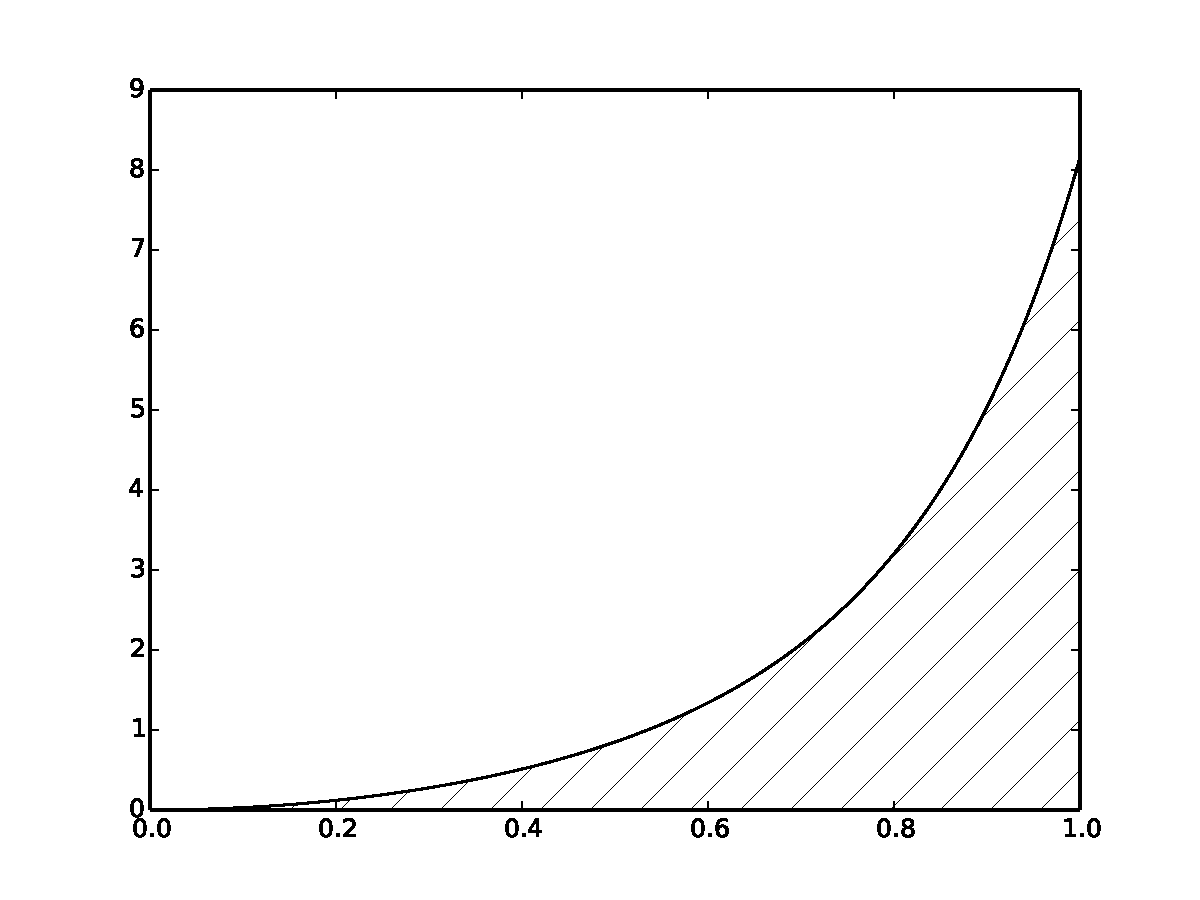
\includegraphics[width=0.7\linewidth]{imgs/integral_of_f.pdf}}
  \caption{
  L'intégrale de $v (t)$ interprétée comme l'aire sous le graphique de $v$. \label{fig:integral_of_f}
  }
\end{figure}
%\clearpage % flush figures fig:integral_of_f


Si nous remplaçons le vrai graphique de la figure~\ref{fig:integral_of_f} par un ensemble de segments de ligne droite, nous pouvons voir la zone plutôt comme composée de trapèzes, dont les zones sont faciles à calculer. Ceci est illustré sur la figure~\ref{fig:viz_trapezoidal}, où 4 segments de ligne droite donnent naissance à 4 trapèzes, couvrant les intervalles de temps $[0,0.2)$, $[0.2,0.6)$, $[0.6,0.8)$ et $[0.8,1.0]$. Notez que nous en avons profité pour démontrer les calculs avec des intervalles de temps de tailles différentes.

\begin{figure}[!ht]  % fig:viz_trapezoidal
  \centerline{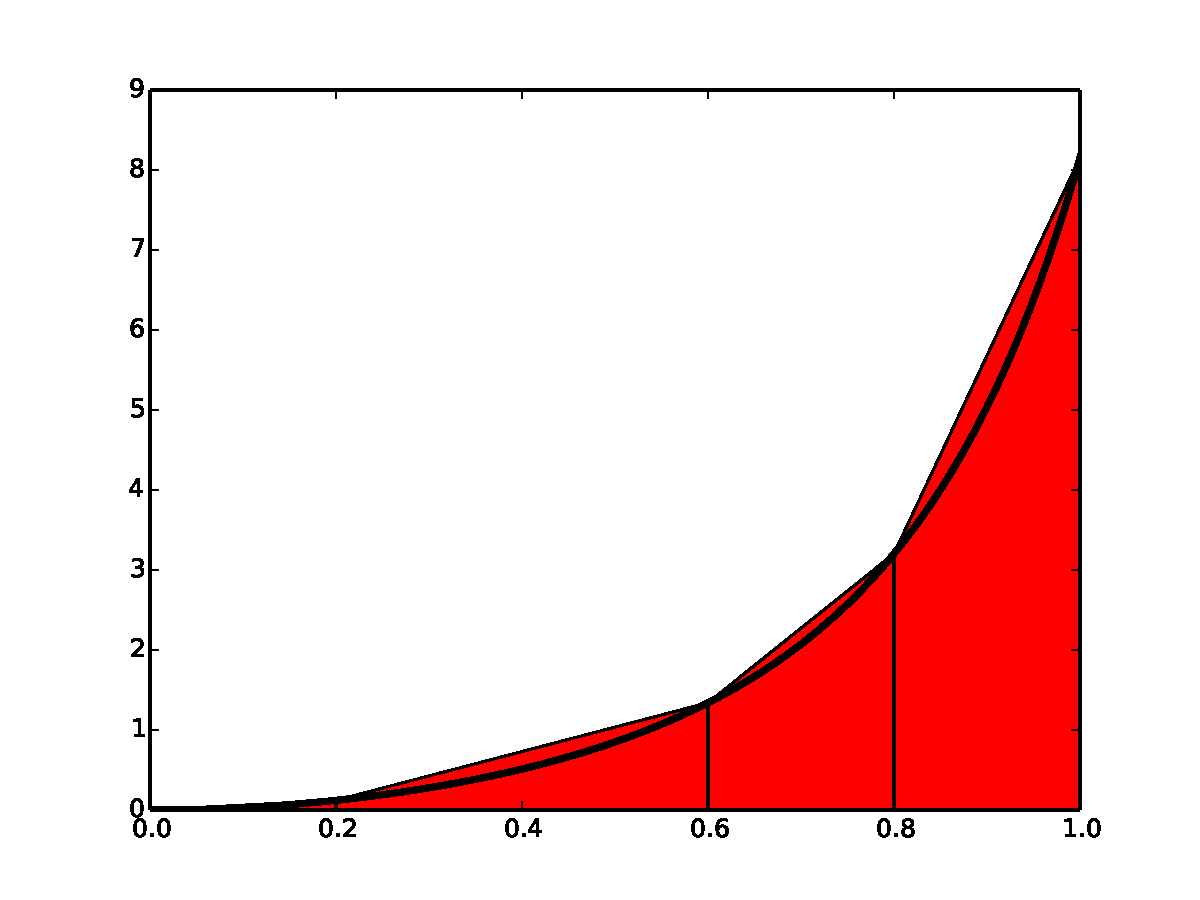
\includegraphics[width=0.7\linewidth]{imgs/viz_trapezoidal.pdf}}
  \caption{
  Calculer approximativement l'intégrale d'une fonction comme la somme des aires des trapèzes. \label{fig:viz_trapezoidal}
  }
\end{figure}
%\clearpage % flush figures fig:viz_trapezoidal

Les aires des 4 trapèzes représentés sur la figure~\ref{fig:viz_trapezoidal} constituent maintenant notre approximation de l'intégrale (\ref{eq:SpeedIntegral}):
\begin{align}
\int_0^1 v(t)dt &\approx
h_1 (\frac{v(0)+v(0.2)}{2}) + h_2 (\frac{v(0.2)+v(0.6)}{2}) \nonumber  \\
&+ h_3 (\frac{v(0.6)+v(0.8)}{2}) + h_4 (\frac{v(0.8)+v(1.0)}{2})
\label{eq:trapezoids}
\end{align}
où
\begin{align}
h_1 &= (0.2 - 0.0) \label{eq:h1}\\
h_2 &= (0.6 - 0.2)  \label{eq:h2}\\
h_3 &= (0.8 - 0.6)  \label{eq:h3}\\
h_4 &= (1.0 - 0.8) \label{eq:h4}
\end{align}
Avec $v(t) = 3t^{2}e^{t^3}$, chaque terme dans (\ref{eq:trapezoids}) est facilement calculé et notre calcul approximatif donne
\begin{equation}
\int_0^1 v(t)dt \approx 1.895
\end{equation}
Par rapport à la vraie réponse de $1.718$, cela est d'environ $10 \%$. Cependant, notez que nous avons utilisé seulement 4 trapèzes pour approximer la zone. Avec plus de trapèzes, l'approximation serait devenue meilleure, puisque les segments de droite du côté supérieur des trapèzes suivraient alors le graphique de plus près. Faire un autre calcul avec plus de trapèzes n'est pas trop tentant pour un humain paresseux, mais c'est un travail parfait pour un ordinateur! Dérivons donc les expressions d'approximation de l'intégrale par un nombre arbitraire de trapèzes.
\subsection{La formule générale}
Pour une fonction donnée $f (x)$, nous voulons approximer l'intégrale $\int_a^bf(x)dx$ par $n$ trapèzes (de largeur égale). Nous commençons par (\ref{eq:SumIntegrals}) et approchons chaque intégrale du côté droit avec un seul trapèze. En détail,
\begin{align}
\int_a^b f(x)\,dx &= \int_{x_0}^{x_1} f(x) dx + \int_{x_1}^{x_2} f(x) dx + \ldots + \int_{x_{n-1}}^{x_n} f(x) dx,     \nonumber \\
                  &\approx h \frac{f(x_0) + f(x_1)}{2} +
		  h \frac{f(x_1) + f(x_2)}{2} + \ldots + \nonumber \\
		  &\quad h \frac{f(x_{n-1}) + f(x_n)}{2} \label{eq:SumTrapezes}
\end{align}
En simplifiant le côté droit de (\ref{eq:SumTrapezes}), nous obtenons
\begin{equation}
\int_a^b f(x)\,dx \approx \\
\frac{h}{2}\left[f(x_0) + 2 f(x_1) + 2 f(x_2) + \ldots + 2 f(x_{n-1}) + f(x_n)\right]
\end{equation}
qui est écrit de façon plus compacte comme
\begin{equation} \label{eq:GenralIntegral}
\int_a^b f(x)\,dx \approx h \left[\frac{1}{2}f(x_0) + \sum_{i=1}^{n-1}f(x_i) + \frac{1}{2}f(x_n) \right]
\end{equation}

\begin{notice_grayiconadmon}[Règles d'intégration composites]
Le mot composite est souvent utilisé lorsqu'une méthode d'intégration numérique est appliquée avec plus d'un sous-intervalle.
à vrai dire alors, écrire, par exemple, "la méthode du trapèze", devrait impliquer l'utilisation d'un seul trapèze, tandis que "la méthode du trapèze composite" est le nom le plus correct lorsque plusieurs trapèzes sont utilisés. Cependant, cette convention de dénomination n'est pas toujours suivie, donc dire que "la méthode du trapèze" peut pointer vers un seul trapèze ainsi que la règle composite avec de nombreux trapèzes.
\end{notice_grayiconadmon} % title: Règles d'intégration composites


\subsection{Implémentation}
\paragraph{Implémentation spécifique ou générale?}
Supposons que notre objectif principal était de calculer l'intégrale spécifique $\int_0^1 v(t)dt$ avec $v(t)=3t^2e^{t^3}$. D'abord, nous avons joué avec un simple calcul de main pour voir de quoi il s'agissait, avant de développer (comme c'est souvent le cas en mathématiques) une formule générale (\ref{eq:GenralIntegral}) pour l'intégrale générale ou «abstraite» $\int_a^bf(x)dx$. Pour résoudre notre problème spécifique $\int_0^1 v(t)dt$, nous devons ensuite appliquer la formule générale (\ref{eq:GenralIntegral}) aux données données (fonction et limites intégrales) dans notre problème. Bien que simples en principe, les étapes pratiques sont déroutantes pour beaucoup car la notation dans le problème abstrait de (\ref{eq:GenralIntegral}) diffère de la notation dans notre problème spécial. Clairement, les $f$, $x$ et $h$ dans (\ref{eq:GenralIntegral}) correspondent à $v$, $t$ et peut-être $\Delta t$ pour la largeur du trapèze dans notre problème spécial.

\begin{question_grayiconadmon}[Le dilemme du programmeur]
\begin{enumerate}
\item Faut-il écrire un programme spécial pour l'intégrale spéciale, en utilisant les idées de la règle générale (\ref{eq:GenralIntegral}), mais en remplaçant $f$ par $v$, $x$ par $t$ et $h$ par $\Delta t$?

\item Faut-il implémenter la méthode générale (\ref{eq:GenralIntegral}) telle qu'elle se présente dans une fonction générale \texttt{trapeze(f, a, b, n)} et résoudre le problème spécifique en question par un appel spécialisé à cette fonction?
\end{enumerate}

\noindent
\textbf{L'alternative 2 est toujours le meilleur choix!}
\end{question_grayiconadmon} % title: Le dilemme du programmeur



La première alternative dans l'encadré ci-dessus semble moins abstraite et donc plus attrayante pour beaucoup. Néanmoins, comme nous l'espérons, cela sera évident à partir des exemples, la deuxième alternative est en fait la plus simple et la plus fiable d'un point de vue mathématique et de programmation. Ces auteurs affirmeront que la deuxième alternative est l'essence même du pouvoir des mathématiques, tandis que la première alternative est la source de beaucoup de confusion sur les mathématiques!
\paragraph{Implémentation avec fonctions.}
Pour l'intégrale $\int_a^bf(x)dx$ calculée par la formule (\ref{eq:GenralIntegral}), nous voulons que le trapèze de la fonction Python correspondante prenne tout $f$, $a$, $b$ et $n$ en entrée et renvoie l'approximation à l'intégrale.

Nous écrivons une fonction Python \texttt{trapeze()} dans un fichier \Verb!trapeze_integral.py! aussi proche que possible de la formule (\ref{eq:GenralIntegral}), en nous assurant que les noms de variables correspondent à la notation mathématique:

\begin{cod}{cbg_gray}\begin{minted}[fontsize=\fontsize{9pt}{9pt},linenos=false,mathescape,baselinestretch=1.0,fontfamily=tt,xleftmargin=2mm]{python}
## NOM DU PROGRAMME: trapeze_integral.py
def trapeze(f, a, b, n):
    h = (b-a)/n
    result = 0.5*f(a) + 0.5*f(b)
    for i in range(1, n):
        xi = a + i*h
        result += f(xi)
    result *= h
    return result
\end{minted}
\end{cod}
\noindent
\paragraph{Résoudre notre problème spécifique en une session.}
Le simple fait d'avoir la fonction \texttt{trapeze()} comme seul contenu d'un fichier \Verb!trapeze_integral.py! fait automatiquement de ce fichier un module que nous pouvons importer et tester dans une session interactive:
\begin{cod}{cbg_gray}\begin{minted}[fontsize=\fontsize{9pt}{9pt},linenos=false,mathescape,baselinestretch=1.0,fontfamily=tt,xleftmargin=2mm]{python}
In [3]: from trapeze_integral import trapeze
In [4]: from math import exp
In [5]: v = lambda t: 3*(t**2)*exp(t**3)
In [6]: n = 4
In [7]: numerical = trapeze(v, 0, 1, n)
In [8]: numerical
Out[8]: 1.9227167504675762
\end{minted}
\end{cod}
\noindent
Calculons l'expression exacte et l'erreur dans l'approximation:
\begin{cod}{cbg_gray}\begin{minted}[fontsize=\fontsize{9pt}{9pt},linenos=false,mathescape,baselinestretch=1.0,fontfamily=tt,xleftmargin=2mm]{python}
In [9]: V = lambda t: exp(t**3) - 1
In [10]: exact = V(1) - V(0)
In [11]: exact - numerical
Out[11]: -0.20443492200853108
\end{minted}
\end{cod}
\noindent
Cette erreur est-elle convaincante? On peut essayer un $n$ plus grand:
\begin{cod}{cbg_gray}\begin{minted}[fontsize=\fontsize{9pt}{9pt},linenos=false,mathescape,baselinestretch=1.0,fontfamily=tt,xleftmargin=2mm]{python}
In [12]: numerical = trapeze(v, 0, 1, n=400)
In [13]: exact - numerical
Out[13]: -2.1236490512777095e-05
\end{minted}
\end{cod}
\noindent
Heureusement, beaucoup plus de trapèzes donnent une erreur beaucoup plus petite.
\paragraph{Résoudre notre problème spécifique dans un programme.}
Au lieu de calculer notre problème spécial dans une session interactive, nous pouvons le faire dans un programme. Comme toujours, un morceau de code faisant une chose particulière est mieux isolé en tant que fonction même si nous ne voyons aucune raison future d'appeler la fonction plusieurs fois et même si nous n'avons pas besoin d'arguments pour paramétrer ce qui se passe à l'intérieur de la fonction. Dans le cas présent, nous mettons simplement les instructions que nous aurions autrement mises dans un programme principal, à l'intérieur d'une fonction:

\begin{cod}{cbg_gray}\begin{minted}[fontsize=\fontsize{9pt}{9pt},linenos=false,mathescape,baselinestretch=1.0,fontfamily=tt,xleftmargin=2mm]{python}
def application():
    from math import exp
    v = lambda t: 3*(t**2)*exp(t**3)
    n = int(input('n: '))
    numerical = trapeze(v, 0, 1, n)

    # Comparer avec le résultat exact
    V = lambda t: exp(t**3) - 1
    exact = V(1) - V(0)
    print(exact)
    error = exact - numerical
    print('n=%d: %.16f, erreur: %g' % (n, numerical, error))
\end{minted}
\end{cod}
\noindent

Maintenant, nous calculons notre problème spécial en appelant \texttt{application()} comme la seule instruction du programme principal.

\paragraph{Faire un module.}
Lorsque nous avons les différentes parties de notre programme comme une collection de fonctions, il est très simple de créer un \emph{module} qui peut être importé dans d'autres programmes. Ce fait, avoir notre code comme module, signifie que la fonction \texttt{trapeze()} peut facilement être réutilisée par d'autres programmes pour résoudre d'autres problèmes. Les exigences d'un module sont simples: mettez tout à l'intérieur des fonctions et laissez les appels de fonction dans le programme principal être dans le soi-disant \emph{bloc de test}:
\begin{cod}{cbg_gray}\begin{minted}[fontsize=\fontsize{9pt}{9pt},linenos=false,mathescape,baselinestretch=1.0,fontfamily=tt,xleftmargin=2mm]{python}
if __name__ == '__main__':
    application()
\end{minted}
\end{cod}
\noindent

Le test \texttt{if} est vrai si le fichier de module, \Verb!trapeze_integral.py!, est exécuté en tant que programme et faux si le module est importé dans un autre programme. Par conséquent, lorsque nous effectuons une importation: \Verb!from trapeze_integral import trapeze! dans un fichier, le test échoue et \texttt{application()} n'est pas appelée, c'est-à-dire que notre problème spécial n'est pas résolu et n'imprime rien à l'écran. D'un autre côté, si nous exécutons \Verb!trapeze_integral.py! dans la fenêtre du terminal, la condition de test est positive, \texttt{application()} est appelée et nous obtenons une sortie dans la fenêtre:

\begin{cod}{cbg_gray}\begin{minted}[fontsize=\fontsize{9pt}{9pt},linenos=false,mathescape,baselinestretch=1.0,fontfamily=tt,xleftmargin=2mm]{text}
Terminal> python trapeze_integral.py
n: 400
n=400: 1.7183030649495579, error: -2.12365e-05
\end{minted}
\end{cod}
\noindent
\section{La méthode du point milieu composite}
\subsection{L'idée}
Plutôt que d'approximer l'aire sous une courbe par des trapèzes, nous pouvons utiliser des rectangles simples. Il peut sembler moins précis d'utiliser des lignes horizontales et non des lignes obliques suivant la fonction à intégrer, mais une méthode d'intégration basée sur des rectangles (la méthode du point milieu) est en fait légèrement plus précise que celle basée sur des trapèzes!

Dans la méthode du milieu, nous construisons un rectangle pour chaque sous-intervalle où la hauteur est égale à $f$ au milieu du sous-intervalle. Faisons-le pour quatre rectangles, en utilisant les mêmes sous-intervalles que nous avions pour les calculs manuels avec la méthode du trapèze: $[0,0.2)$, $[0.2,0.6)$, $[0.6,0.8)$ et $[0.8,1.0]$. On a
\begin{align}
\int_0^1 f(t)dt &\approx
   h_1 f\left(\frac{0 + 0.2}{2}\right) +
   h_2 f\left(\frac{0.2 + 0.6}{2}\right) \nonumber  \\
&+ h_3 f\left(\frac{0.6 + 0.8}{2}\right) +
   h_4 f\left(\frac{0.8 + 1.0}{2}\right)
\end{align}
où $h_1$, $h_2$, $h_3$ et $h_4$ sont les largeurs des sous-intervalles, utilisées précédemment avec la méthode du trapèze et définies dans (\ref{eq:h1})-(\ref{eq:h4}).


\begin{figure}[!ht]  % fig:viz_midpoint
  \centerline{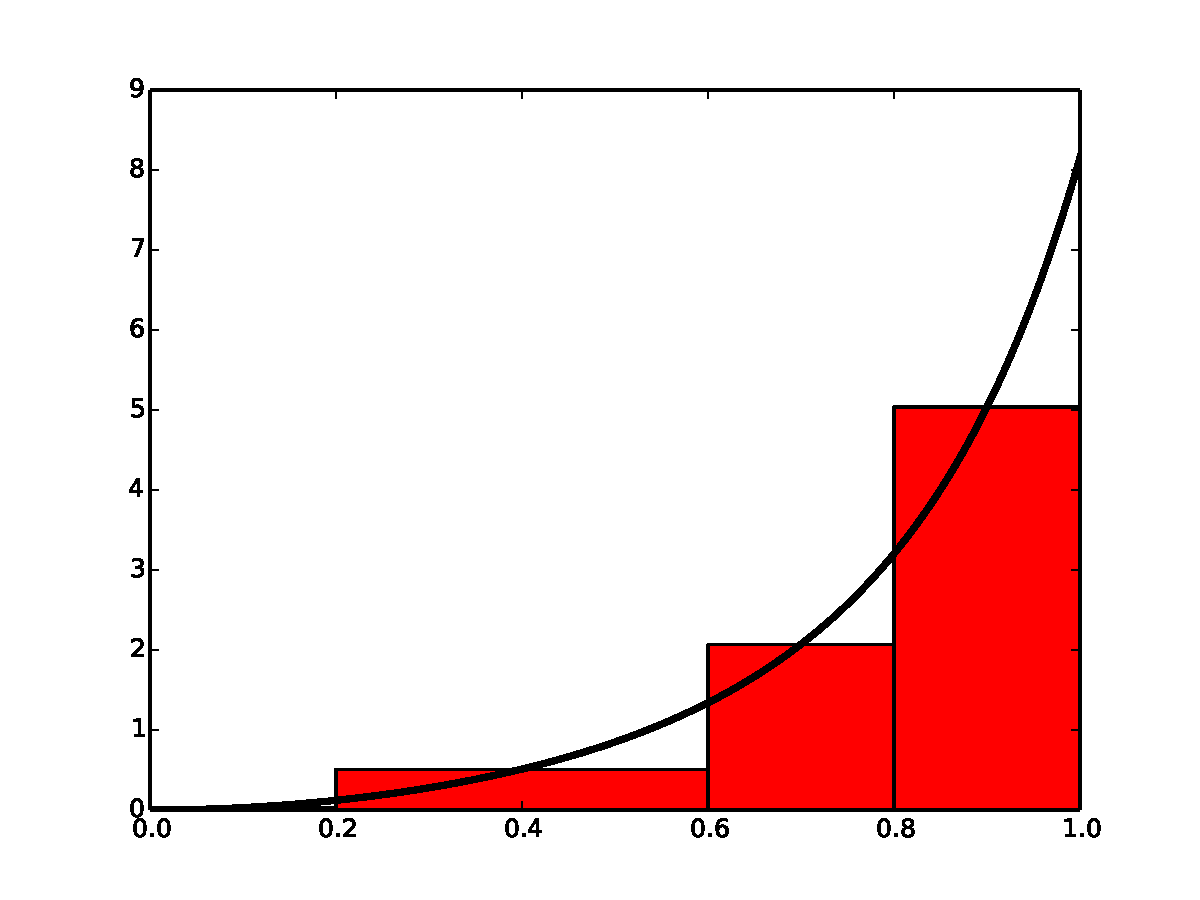
\includegraphics[width=0.7\linewidth]{imgs/viz_midpoint.pdf}}
  \caption{
  Calcul approximatif de l'intégrale d'une fonction comme la somme des aires des rectangles. \label{fig:viz_midpoint}
  }
\end{figure}
%\clearpage % flush figures fig:viz_midpoint


Avec $f(t) = 3t^{2}e^{t^3}$, l'approximation devient $1.632$. Comparé à la vraie réponse ($1.718$), c'est environ $5 \%$ trop petit, mais c'est mieux que ce que nous avons obtenu avec la méthode trapézoïdale ($10 \%$) avec les mêmes sous-intervalles. Plus de rectangles donnent une meilleure approximation.

\subsection{La formule générale}
Dérivons une formule pour la méthode du milieu basée sur $n$ rectangles d'égale largeur:
\begin{align}
\int_a^b f(x)\,dx &= \int_{x_0}^{x_1} f(x)dx + \int_{x_1}^{x_2} f(x)dx +
                     \ldots + \int_{x_{n-1}}^{x_n} f(x)dx,     \nonumber \\
                  &\approx h f\left(\frac{x_0 + x_1}{2}\right) +
                   h f\left(\frac{x_1 + x_2}{2}\right) + \ldots +
                   h f\left(\frac{x_{n-1} + x_n}{2}\right) \\
                  &\approx h \left(f\left(\frac{x_0 + x_1}{2}\right) +
                  f\left(\frac{x_1 + x_2}{2}\right) + \ldots +
                  f\left(\frac{x_{n-1} + x_n}{2}\right)\right)
\end{align}
Cette somme peut être écrite de façon plus compacte comme
\begin{equation} \label{eq:GeneralMidpoint}
\int_a^b f(x) dx \approx h \sum_{i=0}^{n-1}f(x_i)
\end{equation}
où $x_i = \left(a + \frac{h}{2}\right) + ih$.

\subsection{Implémentation}
\label{sec:implementation}
Nous suivons les conseils et les enseignements tirés de l'implémentation de la méthode trapèze et réalisons une fonction \texttt{midpoint(f, a, b, n)} (dans un fichier \Verb!midpoint_integral.py!) pour implémenter la formule générale (\ref{eq:GeneralMidpoint}):

\begin{cod}{cbg_gray}\begin{minted}[fontsize=\fontsize{9pt}{9pt},linenos=false,mathescape,baselinestretch=1.0,fontfamily=tt,xleftmargin=2mm]{python}
## NOM DU PROGRAMME: midpoint_integral.py
def midpoint(f, a, b, n):
    h = float(b-a)/n
    result = 0
    for i in range(n):
        xi = (a + h/2.0) + i*h
        result += f(xi)
    result *= h
    return result
\end{minted}
\end{cod}
\noindent

Nous pouvons tester la fonction comme nous l'avons expliqué pour la méthode du trapèze similaire. L'erreur dans notre problème particulier $\int_0^1 3t^2e^{t^3}dt$ avec quatre intervalles est maintenant d'environ $0.1$ contrairement à $0.2$ pour la règle du trapèze. Les différences sont rarement d'une importance pratique, et sur un ordinateur portable, nous pouvons facilement utiliser $n = 10^6$ et obtenir la réponse avec une erreur d'environ $10^{-12}$ en quelques secondes.
\subsection{Comparaison des méthodes du trapèze et du point milieu}
L'exemple suivant montre la facilité avec laquelle nous pouvons combiner les fonctions \texttt{trapeze()} et \texttt{midpoint()} pour comparer les deux méthodes dans le fichier \Verb!compare_integration_methods.py!:

\begin{pro}{cbg_gray}{bar_gray}\begin{minted}[fontsize=\fontsize{9pt}{9pt},linenos=false,mathescape,baselinestretch=1.0,fontfamily=tt,xleftmargin=2mm]{python}
## NOM DU PROGRAMME: compare_integration_methods.py
#% IMPORTATION
from trapeze_integral import trapeze
from midpoint_integral import midpoint
from math import exp

g = lambda y: exp(-y**2)
a = 0
b = 2
print("      n      point milieu     trapèze")
for i in range(1, 21):
    n = 2**i
    m = midpoint(g, a, b, n)
    t = trapeze(g, a, b, n)
    print('%7d %.16f %.16f'%(n, m, t))
\end{minted}
\end{pro}
\noindent

Notez les efforts mis en forme agréable - la sortie devient
\begin{cod}{cbg_gray}\begin{minted}[fontsize=\fontsize{9pt}{9pt},linenos=false,baselinestretch=1.0,fontfamily=tt,xleftmargin=2mm]{text}
      n      point milieu     trapèze
      2 0.8842000076332692 0.8770372606158094
      4 0.8827889485397279 0.8806186341245393
      8 0.8822686991994210 0.8817037913321336
     16 0.8821288703366458 0.8819862452657772
     32 0.8820933014203766 0.8820575578012112
     64 0.8820843709743319 0.8820754296107942
    128 0.8820821359746071 0.8820799002925637
    256 0.8820815770754198 0.8820810181335849
    512 0.8820814373412922 0.8820812976045025
   1024 0.8820814024071774 0.8820813674728968
   2048 0.8820813936736116 0.8820813849400392
   4096 0.8820813914902204 0.8820813893068272
   8192 0.8820813909443684 0.8820813903985197
  16384 0.8820813908079066 0.8820813906714446
  32768 0.8820813907737911 0.8820813907396778
 131072 0.8820813907631487 0.8820813907610036
 262144 0.8820813907625702 0.8820813907620528
 524288 0.8820813907624605 0.8820813907623183
1048576 0.8820813907624268 0.8820813907623890
\end{minted}
\end{cod}
\noindent
Une inspection visuelle des chiffres montre à quelle vitesse les chiffres se stabilisent dans les deux méthodes. Il semble que 13 chiffres se soient stabilisés dans les deux dernières lignes.


\begin{notice_grayiconadmon}[Remarque]
Les méthodes du trapèze et du point milieu ne sont que deux exemples dans une jungle de règles d'intégration numérique. D'autres méthodes célèbres sont la règle de Simpson et la quadrature de Gauss. Ils fonctionnent tous de la même manière:
$$\int_a^b f(x)dx \approx \sum_{i=0}^{n-1} w_if(x_i)$$
Autrement dit, l'intégrale est approximée par une somme d'évaluations de fonctions, où chaque évaluation $f (x_i)$ reçoit un poids $w_i$. Les différentes méthodes diffèrent par la façon dont elles construisent les points d'évaluation $x_i$ et les poids $w_i$. Nous avons utilisé des points $x_i$ également espacés, mais une précision plus élevée peut être obtenue en optimisant l'emplacement de $x_i$.
\end{notice_grayiconadmon} % title: Remarque



% ======= Intégrales doubles et triples =======
% ===== La règle du point milieu pour une double intégrale =====
% \label{sec:midpointDouble}
% Étant donné une intégrale double sur un domaine rectangulaire $[a, b] \times [c, d]$,
% 
% $$\int_a^b \int_c^d f(x,y) dydx$$
% 
% comment approcher cette intégrale par des méthodes numériques?
% === Dérivation via des intégrales unidimensionnelles ===
% Puisque nous savons comment traiter les intégrales à une variable, une approche fructueuse consiste à considérer l'intégrale double comme deux intégrales, chacune à une variable, qui peut être approximée numériquement par les formules unidimensionnelles précédentes. À cette fin, nous introduisons une fonction intermédiaire $g (x)$ et écrivons
% $$\int_a^b \int_c^d f(x,y) dydx = \int_a^b g(x)dx,\quad
% g(x) = \int_c^d f(x,y) dy$$
% Chacune des intégrales
% $$ \int_a^b g(x)dx,\quad
% g(x) = \int_c^d f(x,y) dy$$
% peut être discrétisé par n'importe quelle règle d'intégration numérique pour une intégrale dans une variable. Utilisons la méthode du point milieu (\ref{eq:GeneralMidpoint}) et commençons par $g(x)=\int_c^d f(x,y)dy$. Nous introduisons $n_y$ intervalles sur $[c, d]$ de longueur $h_y$. La règle du point milieu pour cette intégrale devient alors
% $$g(x) = \int_c^d f(x,y) dy \approx  h_y \sum_{j=0}^{n_y-1} f(x,y_j),
% \quad y_j = c + \frac{1}{2}{h_y} + jh_y $$
% 
% L'expression semble quelque peu différente de (\ref{eq:GeneralMidpoint}), mais c'est à cause de la notation: puisque nous nous intégrons dans la direction $y$ et que nous devrons travailler avec $x$ et $y$ comme coordonnées, nous devons utiliser $n_y$ pour $n$, $h_y$ pour $h$ et le compteur $i$ est plus naturellement appelé $j$ lors de l'intégration dans $y$. Les intégrales dans la direction $x$ utiliseront $h_x$ et $n_x$ pour $h$ et $n$, et $i$ comme compteur.
% 
% L'intégrale double est $\int_a^b g(x)dx$, qui peut être approximée par la méthode du point milieu:
% $$\int_a^b g(x)dx \approx h_x \sum_{i=0}^{n_x-1} g(x_i),\quad x_i=a + \frac{1}{2}{h_x} + ih_x$$
% 
% En rassemblant les formules, nous arrivons à la méthode du point milieu composite pour une double intégrale:
% !bt
% \begin{align}
% \int_a^b \int_c^d f(x,y) dydx &\approx
% h_x \sum_{i=0}^{n_x-1} h_y \sum_{j=0}^{n_y-1} f(x_i,y_j)\nonumber\\
% &=
% h_xh_y \sum_{i=0}^{n_x-1} \sum_{j=0}^{n_y-1} f(a + \frac{h_x}{2} + ih_x, c + \frac{h_y}{2} + jh_y) \\label{eq:MidpointDouble}
% \end{align}
% % La formule (\ref{eq:MidpointDouble}) peut également être dérivée directement dans le cas bidimensionnel en appliquant l'idée de la méthode du point milieu. Nous divisons le rectangle $[a, b] \times [c, d]$ en $nx \times ny$ cellules de taille égale. L'idée de la méthode du point milieu est d'approximer $f$ par une constante sur chaque cellule et d'évaluer la constante au point médian. La cellule $(i, j)$ occupe la zone
% 
% $$[a+ih_x,a+(i+1)h_x]\times [c+jh_y, c+ (j+1)h_y],$$
% et le milieu est $(x_i, y_j)$ avec
% $$x_i=a + ih_x + \frac{1}{2}{h_x} ,\quad y_j = c + jh_y + \frac{1}{2}{h_y}$$
% L'intégrale sur la cellule est donc $h_xh_y f(x_i,y_j)$, et l'intégrale double totale est la somme sur toutes les cellules, qui n'est rien d'autre que la formule (\ref{eq:MidpointDouble}).
% === Programmation d'une double somme ===
% La formule (\ref{eq:MidpointDouble}) implique une double somme, qui est normalement implémentée sous la forme d'une boucle double. Une fonction Python implémentant (\ref{eq:MidpointDouble}) peut ressembler à
% !bc  pycod
% def midpoint_double1(f, a, b, c, d, nx, ny):
% hx = (b - a)/float(nx)
% hy = (d - c)/float(ny)
% I = 0
% for i in range(nx):
% for j in range(ny):
% xi = a + hx/2 + i*hx
% yj = c + hy/2 + j*hy
% I += hx*hy*f(xi, yj)
% return I
% !ec
% Si cette fonction est stockée dans un fichier de module \Verb!midpoint_double.py!, nous pouvons calculer une intégrale, par exemple, $\int_2^3\int_0^2 (2x + y)dxdy=9$ dans un shell interactif et démontrer que la fonction calcule le bon nombre:
% !bc ipy
% >>> from midpoint_double import midpoint_double1
% >>> def f(x, y):
% ...     return 2*x + y
% ...
% >>> midpoint_double1(f, 0, 2, 2, 3, 5, 5)
% 9.0
% !ec
% === Réutilisation du code pour les intégrales unidimensionnelles ===
% Il est très naturel d'écrire une méthode de point milieu bidimensionnelle comme nous l'avons fait dans la fonction \Verb!midpoint_double1! lorsque nous avons la formule (\ref{eq:MidpointDouble}). Cependant, nous pourrions également demander, tout comme nous l'avons fait en mathématiques, pouvons-nous réutiliser une implémentation bien testée pour les intégrales unidimensionnelles pour calculer les doubles intégrales? Autrement dit, pouvons-nous utiliser la fonction \texttt{midpoint}.
% 
% !bc pycod
% def midpoint(f, a, b, n):
% h = float(b-a)/n
% result = 0
% for i in range(n):
% result += f((a + h/2.0) + i*h)
% result *= h
% return result
% !ec
% 
% de la section~\ref{sec:implementation} "deux fois"? La réponse est oui, si nous pensons comme nous l'avons fait dans les mathématiques: calculer l'intégrale double comme règle du point milieu pour intégrer $g (x)$ et définir $g (x_i)$ en termes d'une règle du point milieu sur $f$ dans la coordonnée $y$.
% !bc pycod
% def midpoint_double2(f, a, b, c, d, nx, ny):
% def g(x):
% return midpoint(lambda y: f(x, y), c, d, ny)
% 
% return midpoint(g, a, b, nx)
% !ec
% L'avantage important de cette implémentation est que nous réutilisons une fonction bien testée pour la règle du point milieu unidimensionnelle standard et que nous appliquons la règle unidimensionnelle exactement comme dans les mathématiques.
% === Vérification via les fonctions de test ===
% Comment tester que nos fonctions pour la double intégrale fonctionnent? Le meilleur test unitaire consiste à trouver un problème où l'erreur d'approximation numérique disparaît, car alors nous savons exactement quelle devrait être la réponse numérique. La règle du point milieu est exacte pour les fonctions linéaires, quel que soit le nombre de sous-intervalles que nous utilisons. De plus, toute fonction linéaire bidimensionnelle $f(x,y)=px+qy+r$ sera intégrée exactement par la règle point milieu bidimensionnelle. Nous pouvons choisir $f(x,y)=2x+y$ et créer une fonction de test appropriée qui peut automatiquement vérifier nos deux implémentations alternatives de la règle du point milieu bidimensionnelle. La fonction de test devient:
% !bc pycod
% def test_midpoint_double():
% """Test that a linear function is integrated exactly."""
% def f(x, y):
% return 2*x + y
% 
% a = 0;  b = 2;  c = 2;  d = 3
% import sympy
% x, y = sympy.symbols('x  y')
% I_expected = sympy.integrate(f(x, y), (x, a, b), (y, c, d))
% # Test three cases: nx < ny, nx = ny, nx > ny
% for nx, ny in (3, 5), (4, 4), (5, 3):
% I_computed1 = midpoint_double1(f, a, b, c, d, nx, ny)
% I_computed2 = midpoint_double2(f, a, b, c, d, nx, ny)
% tol = 1E-14
% #print I_expected, I_computed1, I_computed2
% assert abs(I_computed1 - I_expected) < tol
% assert abs(I_computed2 - I_expected) < tol
% !ec
% !bnotice Laisser parler les fonctions de test?
% Si nous appelons la fonction \Verb!test_midpoint_double! ci-dessus et que rien ne se passe, nos implémentations sont correctes. Cependant, il est quelque peu ennuyeux d'avoir une fonction complètement silencieuse lorsqu'elle fonctionne sommes-nous sûrs que tout est correctement calculé? Pendant le développement, il est donc fortement recommandé d'insérer une instruction d'impression afin que nous puissions surveiller les calculs et être convaincu que la fonction de test fait ce que nous voulons. Puisqu'une fonction de test ne doit avoir aucune instruction print(), nous la commentons simplement comme nous l'avons fait dans la fonction listée ci-dessus.
% 
% !enotice
% La méthode du trapèze peut être utilisée comme alternative à la méthode du point milieu. La dérivation d'une formule pour la double intégrale et les implémentations suivent exactement les mêmes idées que nous avons expliquées avec la méthode du point milieu, mais il y a plus de termes à écrire dans les formules.
% ===== La règle du point milieu pour une triple intégrale =====
% === Théorie ===
% Une fois qu'une méthode qui fonctionne pour un problème unidimensionnel est généralisée à deux dimensions, il est généralement assez simple d'étendre la méthode à trois dimensions. Cela sera maintenant démontré pour les intégrales. Nous avons la triple intégrale:
% $$\int_{a}^{b} \int_c^d \int_e^f g(x,y,z) dzdydx$$
% et veulent approximer l'intégrale par une règle du point milieu. En suivant les idées de la double intégrale, nous avons divisé cette intégrale en intégrales unidimensionnelles:
% !bt
% \begin{align*}
% p(x,y) &= \int_e^f g(x,y,z) dz\\
% q(x) &= \int_c^d p(x,y) dy\\
% \int_{a}^{b} \int_c^d \int_e^f g(x,y,z) dzdydx &= \int_a^b q(x)dx
% \end{align*}
% % Pour chacune de ces intégrales unidimensionnelles, nous appliquons la règle du point milieu:
% !bt
% \begin{align*}
% p(x,y) = \int_e^f g(x,y,z) dz
% &\approx \sum_{k=0}^{n_z-1} g(x,y,z_k),
% \\
% q(x) = \int_c^d p(x,y) dy
% &\approx \sum_{j=0}^{n_y-1} p(x,y_j),
% \\
% \int_{a}^{b} \int_c^d \int_e^f g(x,y,z) dzdydx = \int_a^b q(x)dx
% &\approx \sum_{i=0}^{n_x-1} q(x_i),
% \end{align*}
% % où
% $$z_k=e + \frac{1}{2}h_z + kh_z,\quad y_j=c + \frac{1}{2}h_y + jh_y \quad
% x_i=a + \frac{1}{2}h_x + ih_x$$
% En commençant par la formule pour $\int_{a}^{b} \int_c^d \int_e^f g(x,y,z) dzdydx$ et en insérant les deux formules précédentes donne
% !bt
% \begin{align}
% & \int_{a}^{b} \int_c^d \int_e^f g(x,y,z)\, dzdydx\approx\nonumber\\
% & h_xh_yh_z
% \sum_{i=0}^{n_x-1}\sum_{j=0}^{n_y-1}\sum_{k=0}^{n_z-1}
% g(a + \frac{1}{2}h_x + ih_x,
% c + \frac{1}{2}h_y + jh_y,
% e + \frac{1}{2}h_z + kh_z) \\label{eq:midpointTriple}
% \end{align}
% % Notez que nous pouvons appliquer les idées sous Dérivation directe à la fin de la section~\ref{sec:midpointDouble} arrive à (\ref{eq:midpointTriple}) directement: diviser le domaine en $n_x\times n_y\times n_z$ cellules de volumes $h_xh_yh_z$; approximativement g par une constante, évaluée au milieu $(x_i,y_j,z_k)$, dans chaque cellule; et additionner les intégrales de cellule $h_xh_yh_zg(x_i,y_j,z_k)$.
% === Implémentation ===
% Nous suivons les idées pour les implémentations de la règle du point milieu pour une double intégrale. Les fonctions correspondantes sont présentées ci-dessous et se trouvent dans le fichier \Verb!midpoint_triple.py!.
% !bc pycod
% def midpoint_triple1(g, a, b, c, d, e, f, nx, ny, nz):
% hx = (b - a)/float(nx)
% hy = (d - c)/float(ny)
% hz = (f - e)/float(nz)
% I = 0
% for i in range(nx):
% for j in range(ny):
% for k in range(nz):
% xi = a + hx/2 + i*hx
% yj = c + hy/2 + j*hy
% zk = e + hz/2 + k*hz
% I += hx*hy*hz*g(xi, yj, zk)
% return I
% 
% def midpoint(f, a, b, n):
% h = float(b-a)/n
% result = 0
% for i in range(n):
% result += f((a + h/2.0) + i*h)
% result *= h
% return result
% 
% def midpoint_triple2(g, a, b, c, d, e, f, nx, ny, nz):
% def p(x, y):
% return midpoint(lambda z: g(x, y, z), e, f, nz)
% 
% def q(x):
% return midpoint(lambda y: p(x, y), c, d, ny)
% 
% return midpoint(q, a, b, nx)
% 
% def test_midpoint_triple():
% """Test that a linear function is integrated exactly."""
% def g(x, y, z):
% return 2*x + y - 4*z
% 
% a = 0;  b = 2;  c = 2;  d = 3;  e = -1;  f = 2
% import sympy
% x, y, z = sympy.symbols('x y z')
% I_expected = sympy.integrate(
% g(x, y, z), (x, a, b), (y, c, d), (z, e, f))
% for nx, ny, nz in (3, 5, 2), (4, 4, 4), (5, 3, 6):
% I_computed1 = midpoint_triple1(
% g, a, b, c, d, e, f, nx, ny, nz)
% I_computed2 = midpoint_triple2(
% g, a, b, c, d, e, f, nx, ny, nz)
% tol = 1E-14
% print(I_expected, I_computed1, I_computed2)
% assert abs(I_computed1 - I_expected) < tol
% assert abs(I_computed2 - I_expected) < tol
% 
% if __name__ == '__main__':
% test_midpoint_triple()
% !ec

\section{Intégration Monte Carlo}
Les méthodes de Monte Carlo sont des techniques de calcul probabilistes. Au cœur, un algorithme de Monte Carlo représente de façon aléatoire certaines valeurs de l'espace de valeurs d'un paramètre considéré. La combinaison de plusieurs paramètres permet de tirer des conclusions stochastiques des relations. L'intégration des fonctions mathématiques de la forme:
\begin{equation*}
A = \int_a^b f(x) \cdot dx
\end{equation*}

Pour effectuer une intégration, nous voulons savoir comment les valeurs sélectionnées au hasard sont réparties: lesquelles des valeurs sont égales ou inférieures à la valeur de la fonction et lesquelles sont supérieures. Il s'agit d'une décision binaire qui divise les valeurs aléatoires en deux groupes. Du rapport de la taille des groupes, nous pouvons tirer nos conclusions.

Nous utilisons la fonction (intégrande) comme critère de décision uniquement. L'algorithme ne nous fournit rien d'autre que des comptes/fréquences. La fermeture probabiliste est alors:
\begin{equation*}
\frac{\textrm{cas favorables}} {\textrm{cas possibles}} = \frac {n}{N} = \frac{A_{sous\;la\;fonction}}{A_{aire \;totale}}
\end{equation*}
La zone $A_{sous\;la\;fonction}$ est la zone inconnue qui nous intéresse. Pour $A_{aire \;totale}$, nous choisissons arbitrairement une région simple, cette zone que nous pouvons calculer sans difficultés.

\subsection{Exemple: détermination de $\pi$}
À titre d'exemple, nous choisissons un cercle dont la fonction mathématique est donnée par la première:
\begin{align*}
x^2 + y^2 &= R^2 \\
y = f(x) &= \sqrt{R^2 - x^2}
\end{align*}
Pour l'estimation de $\pi$, l'aire du cercle est comparée à l'aire du carré $2R \times 2R$, ce rapport est $\pi / 4$:
\begin{align*}
A_{cercle} &= R^2 \cdot \pi \\
A_{carré} &= {(2R)}^2 = 4R^2
\end{align*}
Nous générons au hasard $(x_rand, y_rand)$-points. Pour chaque point, nous devons décider s'il se trouve à l'intérieur ou à l'extérieur du cercle. Pour cela, nous utilisons la différence $y_{rand} - f(x_{rand})$, où $f(x) = \sqrt{R^2 - x^2}$ est la fonction d'un cercle dans le premier quadrant. Nous pouvons compter le nombre de points à l'intérieur du cercle. Nous pouvons compter le nombre de points à l'intérieur du cercle. Le rapport $n / N$ est supposé être égal au rapport $A_{cercle}/A_{carré}$
\begin{align*}
\frac {\textrm{n = (x,y)-points dans le cercle}}  {\textrm{N = (x,y)-points dans le carré}} &= \frac{A_{cercle}}{A_{carré}}
 = \frac {R^2 \cdot \pi}{4R^2 } = \frac {\pi}{4} \\
\pi &= 4\frac{n}{N}
\end{align*}
\subsection{implémentation}
Nous avons vu l'intégration de Monte Carlo lorsque nous avons calculé $\pi / 4$ en calculant l'aire du quart de cercle unitaire.

Voici le code:

\begin{pro}{cbg_gray}{bar_gray}\begin{minted}[fontsize=\fontsize{9pt}{9pt},linenos=false,mathescape,baselinestretch=1.0,fontfamily=tt,xleftmargin=2mm]{python}
## NOM DU PROGRAMME: MC_integral.py
#% IMPORTATION
import numpy as np
import matplotlib.pyplot as plt

def f(x):
    '''
    fonction pour un cercle
    '''
    return np.sqrt(1-x*x)

N = 10000   # nombre d'essais
x0 = 0
x1 = 1

x = np.arange(x0, x1, 0.01)
y = f(x)
fmax = max(y)
np.random.seed(6)
x_rand = x0 + (x1 - x0) * np.random.rand(N)
y_rand = fmax * np.random.rand(N)
n = np.sum(y_rand - f(x_rand) < 0.0) # nombre de points dans le cercle
#----- Sortie et graphiques -------------------
print('PI numpy       : ', np.pi)
print('PI monte carlo : ', 4*n/N)
print('différence     : ', 4*n/(N) - np.pi)

index_below = np.where(y_rand < f(x_rand))
index_above = np.where(y_rand >= f(x_rand))
plt.figure(figsize=(7,7))
plt.plot(x,f(x),'--k')
plt.scatter(x_rand[index_below], y_rand[index_below],
            c="r", s = 5, label = "Pts sous la courbe")
plt.scatter(x_rand[index_above], y_rand[index_above],
            c="b", s = 5, label = "Pts au-dessus de la courbe")
plt.legend(bbox_to_anchor=(0., 1.02, 1., .102), ncol=2)
plt.show()
\end{minted}
\end{pro}
\noindent
\begin{cod}{cbg_gray}\begin{minted}[fontsize=\fontsize{9pt}{9pt},linenos=false,mathescape,baselinestretch=1.0,fontfamily=tt,xleftmargin=2mm]{text}
PI numpy       :  3.141592653589793
PI monte carlo :  3.1436
différence     :  0.002007346410207056
\end{minted}
\end{cod}
\noindent


\vspace{6mm}

% inline figure
\centerline{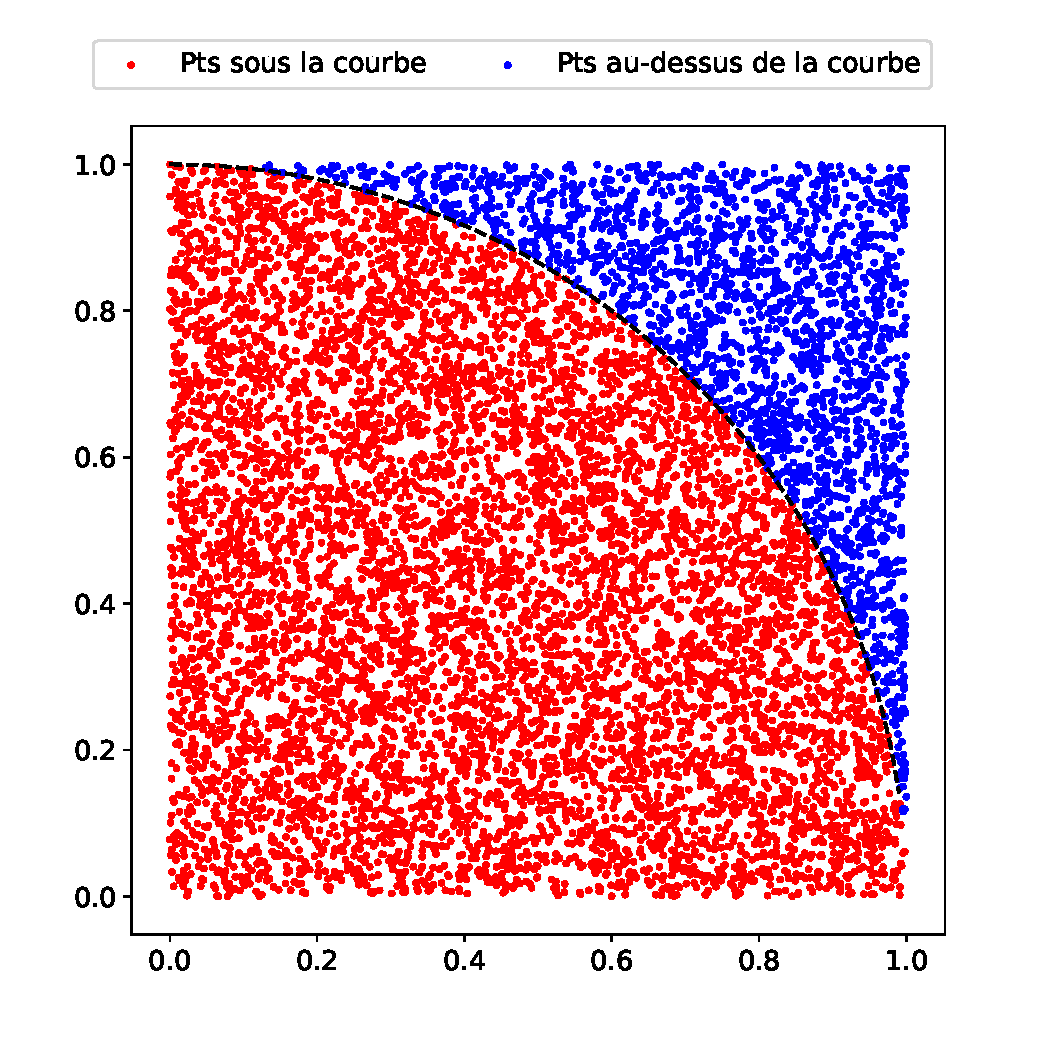
\includegraphics[width=0.7\linewidth]{imgs/MC_integral.pdf}}

\vspace{6mm}



Nous pouvons généraliser cette approche aux courbes autres que $y = \sqrt{1-x^2}$. L'idée est la suivante: pour une courbe arbitraire, trouvez le rectangle qui la contient, générez un point aléatoire dans ce rectangle et déterminez combien de points aléatoires se trouvent sous la courbe.

% ------------------- end of main content ---------------

% #ifdef PREAMBLE
\end{document}
% #endif

